\documentclass{homework}
% \usepackage{lua-visual-debug}
\usepackage{graphicx}
\usepackage{amsmath, amssymb, amsfonts}
\usepackage{enumitem}
\usepackage{ulem}
\usepackage{tikz}
\usepackage[a4paper, total={6in, 8.8in}]{geometry}

\title{Practice \#4}
\subject{CS341 Introduction to Computer Networks}
\studentid{20170058}
\name{Keonwoo Kim}
\date{\today}

\begin{document}
\maketitle

\parindent=0pt


\solution{
    \vspace*{-1.3em}
    \begin{enumerate}[label={1.\arabic*.}, topsep=-2em]
        \item I set the \texttt{width} parameter of the grid to \texttt{5}, and set the \texttt{GridWidth} parameter to \texttt{UintegerValue (size / 2)}. This makes a grid as in the figure.
        \item[1.2.1.] Every pair of two nodes are one hop away.
        \item[1.2.2.] It is because the distances between any two nodes are short enough to be connected directly within a single hop.
        \item[1.3.] The maximum value of the width (the length of AB) such that C and D are still one hop away from each other is \emph{20 m}.
        \item[1.4.] The minimum value of the height (the length of AD) such that ABC are not connected to any of DEF is \emph{52 m}.
    \end{enumerate}
    \vspace*{3.3em}
}

\solution{
    \vspace*{-1.3em}
    \begin{enumerate}[label={2.\arabic*.}, topsep=-2em]
        \item \hfill\\
        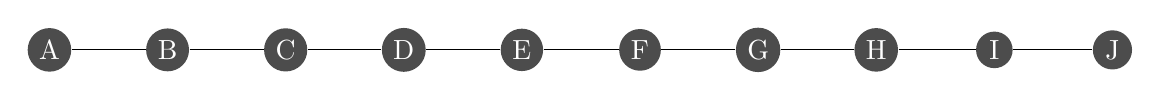
\begin{tikzpicture}[circle/.style={shape=circle,inner sep=2pt,fill=black!70,text=white, minimum width=1em}]
            \path 
            (0, 0) node [circle] (p0) {A}
            (1*1.5, 0) node [circle] (p1) {B}
            (2*1.5, 0) node [circle] (p2) {C}
            (3*1.5, 0) node [circle] (p3) {D}
            (4*1.5, 0) node [circle] (p4) {E}
            (5*1.5, 0) node [circle] (p5) {F}
            (6*1.5, 0) node [circle] (p6) {G}
            (7*1.5, 0) node [circle] (p7) {H}
            (8*1.5, 0) node [circle] (p8) {I}
            (9*1.5, 0) node [circle] (p9) {J};
            \draw (p0) -- (p1) -- (p2) -- (p3) --(p4) -- (p5) -- (p6) -- (p7) -- (p8) -- (p9);
        \end{tikzpicture}
        \item [2.2.1.] \hfill\\
        \includegraphics[width=0.5\textwidth]{task2-1}%
        \includegraphics[width=0.5\textwidth]{task2-2}
        \item [2.2.2.] \hfill\\
        \includegraphics[width=\textwidth]{task2-3}
        \item [2.2.3.] \hfill\\
        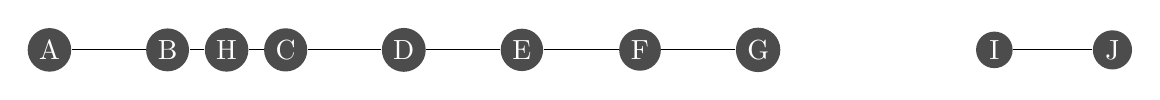
\begin{tikzpicture}[circle/.style={shape=circle,inner sep=2pt,fill=black!70,text=white, minimum width=1em}]
            \path 
            (0, 0) node [circle] (p0) {A}
            (1*1.5, 0) node [circle] (p1) {B}
            (2*1.5, 0) node [circle] (p2) {C}
            (3*1.5, 0) node [circle] (p3) {D}
            (4*1.5, 0) node [circle] (p4) {E}
            (5*1.5, 0) node [circle] (p5) {F}
            (6*1.5, 0) node [circle] (p6) {G}
            (1.5*1.5, 0) node [circle] (p7) {H}
            (8*1.5, 0) node [circle] (p8) {I}
            (9*1.5, 0) node [circle] (p9) {J};
            \draw (p0) -- (p1) -- (p7) -- (p2) -- (p3) --(p4) -- (p5) -- (p6);
            \draw (p8) -- (p9);
        \end{tikzpicture}
        \item [2.2.4.] \hfill\\
        \includegraphics[width=\textwidth]{task2-4}
        There are some table entries whose flags are marked as DOWN which were UP before the change. Since the node J is nearer to the broken part of the network than C, the update of the routing table of $\text{J}\to\text{C}$ should be faster than one of $\text{C}\to\text{J}$. This might be a reason that some of entries are changed to DOWN in $\text{J}\to\text{C}$ table but not in $\text{C}\to\text{J}$.
    \end{enumerate}
    \vspace*{3.3em}
}

\solution{
    \vspace*{-1.3em}
    \begin{enumerate}[label={1.\arabic*.}, topsep=-2em]
        \item [3.1.1.] \hfill\\
        \includegraphics[width=0.9\textwidth]{task3-0}\hfill\\
        \includegraphics[width=0.9\textwidth]{task3-0-1}\hfill\\
        \includegraphics[width=0.9\textwidth]{task3-1}\hfill\\
        \item [3.1.2.] It shows the same route with one in 3.1.1, that is ACEF. There might be other routes such as ABEF or ADEF. Allowing routes with more hop counts, we can think of routes such as ABCEF, ACBEF, or ADBCEF as well. Note, regarding ABEF, ACEF, and ADEF, that there are no differences in hop counts, and ignoring the actual distance and considering only hop counts, the situation of B, C, and D are the same. The distance vector routing protocol selected the node C. This might be because of other factors, such as response time: C responded faster to A than B or D. So the node C is recorded to the routing table faster, and when calculating the hop count of E, it finds C as an intermediate node.
        \item [3.2.1.] \hfill\\
        \includegraphics[width=0.6\textwidth]{task3-2-0}\hfill\\
        \includegraphics[width=0.7\textwidth]{task3-2-1}\hfill\\
        \includegraphics[width=0.9\textwidth]{task3-2}\hfill\\
        Note that the hop counts are significantly different: CBAF is of 3 hops, while CDF is of 2 hops.
        \item [3.2.2.] The path with less hop counts are prioritized, as it makes the route better and reduces the travel time.
        \item [3.2.3.] Since it prioritizes less hop counts, the path A would be selected. The path A is of 1000 hop counts, while the path B is of 1001 hop counts.
        \item [3.2.4.] The route with less hop counts are better in terms of transmission delay, since it passes less routers -- this will be pros of the path A. However, especially in wireless setting, propagation delay might not be negligible and might be comparable with the transmission delay. Also, the error rate might increase as it travels longer distance -- these points could be cons of the path A. Although it will be better to measure pros and cons in reality, the path A will be better assuming passing more routers are significantly worse than other cons.
    \end{enumerate}
    \vspace*{3.3em}
}


\end{document}